\documentclass[aspectratio=169,11pt]{beamer}
% Phase 2 presentation. Compile from this folder: pdflatex slides_phase2 (run twice).
% Figures are read from ../results/figures/ (generated by notebooks 08-11).
% Every number here is taken from results/metrics/ and matches report/phase2.tex.
\usetheme{default}
\usecolortheme{dove}
\setbeamertemplate{navigation symbols}{}
\setbeamertemplate{footline}[frame number]
\usepackage{booktabs}
\usepackage{graphicx}
\graphicspath{{../results/figures/}}
\newcommand{\ugm}{$\mu$g/m$^3$}

\title{One-Hour-Ahead PM2.5 Forecasting: LSTM and an XGBoost--LSTM Hybrid}
\subtitle{Deep learning under the same leakage-controlled protocol as Phase~1}
\author{Animesh Kumar Rai \and Rishiwant Kumar Maurya \and Supreet \and Aditya Shankar \and Drishti Jha}
\institute{Team T051 --- Advance Machine Learning}
\date{Project 19 --- Phase 2}

\begin{document}

\begin{frame}
\titlepage
\end{frame}

\begin{frame}{Recap and the Phase~2 question}
\begin{itemize}
\item \textbf{Phase~1:} a 37-feature XGBoost beat persistence on 2014 (MAE 10.96 vs 11.93 \ugm{}), but only by $\approx 9\%$ --- PM2.5 is 96\% autocorrelated at 1~h.
\item \textbf{Phase~2 question:} instead of hand-made lags, can a \emph{deep} model read the raw hourly history and learn the temporal structure itself?
\item Natural choice: an \textbf{LSTM} (recurrent network for long-range memory).
\item Evaluated under the \emph{identical} protocol and eval hours, so LSTM, XGBoost and the baselines are directly comparable.
\item Bonus: a \textbf{hybrid} of the tree and the network --- does combining help?
\end{itemize}
\end{frame}

\begin{frame}{Input sequences: raw windows, no leakage}
\begin{columns}
\column{0.52\textwidth}
\begin{itemize}
\item For each issuance time $t$: a window of the last \textbf{24 hours}, 14 channels each.
\item Channels: PM2.5 + ``was-missing'' flag, dew point, temperature, pressure, decoded wind speed, one-hot wind direction, snow/rain, hour sin/cos.
\item PM2.5 forward-filled (LSTM cannot read NaN); scaling uses \textbf{training stats only}.
\item \textbf{Leakage check:} corrupting $x_{t+1}$ leaves every input window unchanged (now enforced by a unit test).
\end{itemize}
\column{0.48\textwidth}
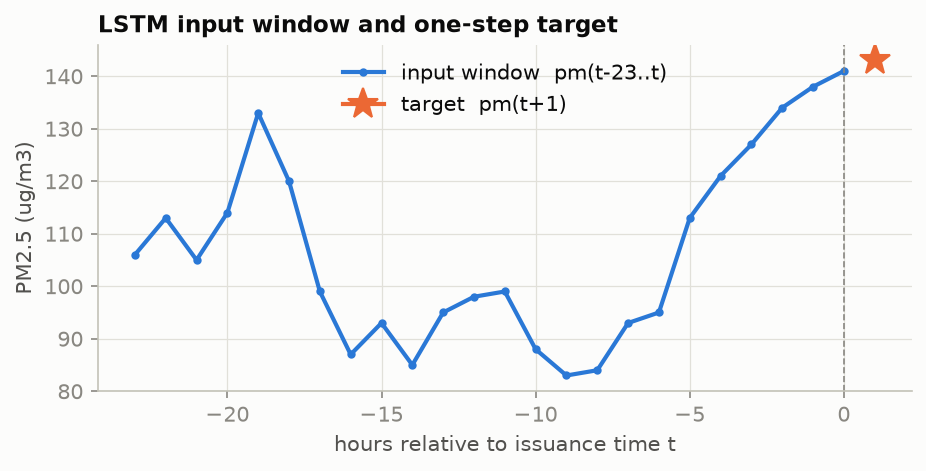
\includegraphics[width=\linewidth]{dl_01_window_example.png}
\end{columns}
\end{frame}

\begin{frame}{LSTM model}
\begin{columns}
\column{0.5\textwidth}
\begin{itemize}
\item 2-layer LSTM, 64 hidden units, dropout, linear output.
\item Predicts the \textbf{change} $x_{t+1}-x_t$, adds $x_t$ back --- an easier target for a persistent series.
\item \textbf{Regularisation:} dropout 0.1, weight decay $10^{-4}$, gradient clipping 1.0, early stopping on a 15\% tail.
\item Adam, lr $10^{-3}$, batch 256, up to 40 epochs; fixed seed.
\end{itemize}
\column{0.5\textwidth}
\begin{tabular}{lc}
\toprule
Setting & Value \\
\midrule
Lookback & 24 h \\
Layers / hidden & 2 / 64 \\
Dropout & 0.1 \\
Target & change $x_{t+1}-x_t$ \\
Weight decay & $10^{-4}$ \\
Batch & 256 \\
\bottomrule
\end{tabular}
\vspace{0.8em}

\footnotesize GPU (Metal/MPS), PyTorch; one fit $\approx$ 17~s.
\end{columns}
\end{frame}

\begin{frame}{Ablation: shorter memory wins}
\begin{columns}
\column{0.55\textwidth}
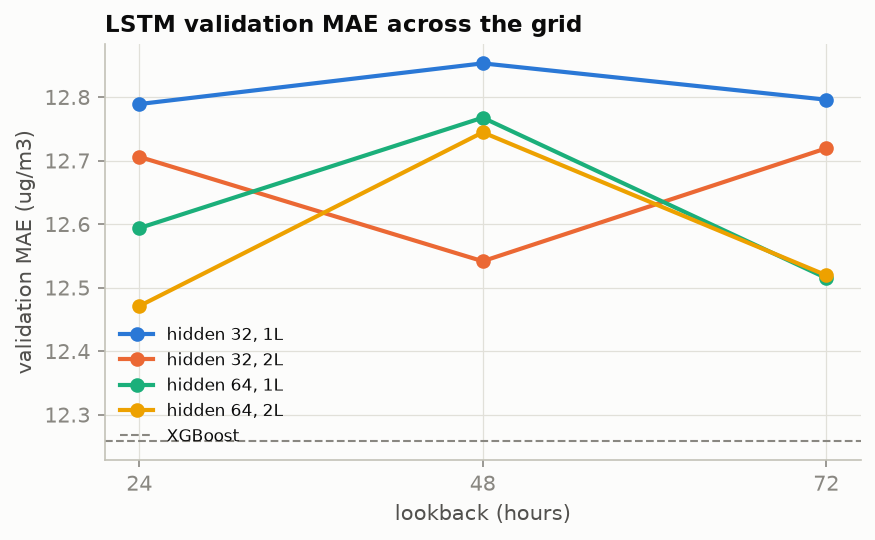
\includegraphics[width=\linewidth]{dl_02_lstm_search.png}
\column{0.45\textwidth}
\begin{itemize}
\item Grid of 12: lookback (24/48/72), hidden (32/64), layers (1/2).
\item \textbf{All 12 beat persistence} (val MAE 13.18).
\item Best is the \emph{shortest} 24-h window; 48/72~h gave no gain.
\item Narrow spread (12.47--12.85 \ugm{}): the LSTM is not sensitive to these choices.
\item Matches Phase~1: only the most recent hours carry signal at 1~h.
\end{itemize}
\end{columns}
\end{frame}

\begin{frame}{Validation (2013): close, but not ahead}
\begin{center}
\begin{tabular}{lccc}
\toprule
Model & MAE & RMSE & $R^2$ \\
\midrule
Persistence & 13.18 & 24.87 & 0.936 \\
XGBoost (change) & \textbf{12.26} & \textbf{22.53} & \textbf{0.947} \\
LSTM & 12.47 & 22.85 & 0.946 \\
\bottomrule
\end{tabular}
\end{center}
\begin{itemize}
\item The LSTM clearly beats persistence, but stays a little behind the tuned XGBoost.
\item Learning from raw history gets \emph{very close} to hand-engineered features --- it does not overtake them.
\end{itemize}
\end{frame}

\begin{frame}{Hybrid: blend two different error patterns}
\begin{columns}
\column{0.48\textwidth}
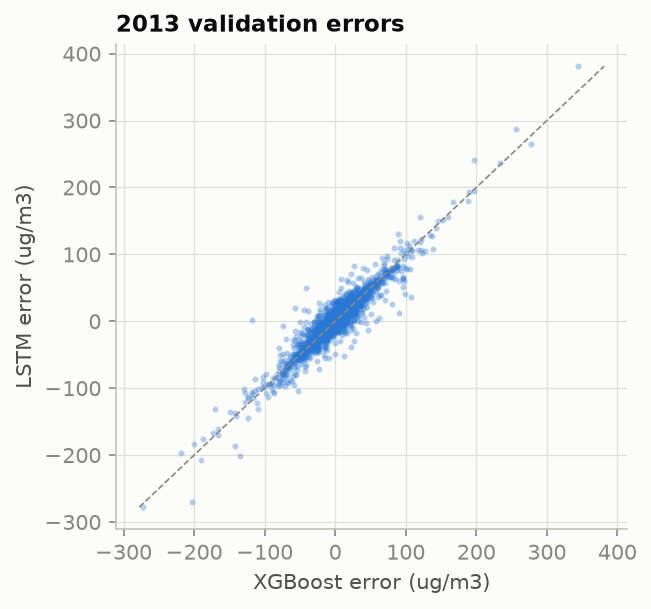
\includegraphics[width=\linewidth]{dl_05_error_scatter.png}
\column{0.52\textwidth}
\begin{itemize}
\item On 2013 the two models' errors correlate at \textbf{0.95} --- similar, but not identical.
\item Convex blend: $\hat{y}=w\,\hat{y}_{\text{xgb}}+(1-w)\,\hat{y}_{\text{lstm}}$.
\item Single weight $w$ chosen by least squares on 2013, then \textbf{frozen} for 2014.
\item Fitted $w = 0.63$ (63\% XGBoost, 37\% LSTM) --- one parameter, hard to overfit.
\end{itemize}
\end{columns}
\end{frame}

\begin{frame}{Test year 2014 (single evaluation)}
\begin{columns}
\column{0.46\textwidth}
\begin{tabular}{lccc}
\toprule
 & MAE & RMSE & $R^2$ \\
\midrule
Persistence & 11.93 & 22.03 & 0.944 \\
XGBoost & 10.96 & 19.96 & 0.954 \\
LSTM & 11.28 & 20.49 & 0.952 \\
\textbf{Hybrid} & \textbf{10.90} & \textbf{19.89} & \textbf{0.955} \\
\bottomrule
\end{tabular}
\vspace{0.6em}
\begin{itemize}
\item Ordering holds from validation.
\item LSTM $>$ persistence; XGBoost $>$ LSTM; hybrid best overall.
\end{itemize}
\column{0.54\textwidth}
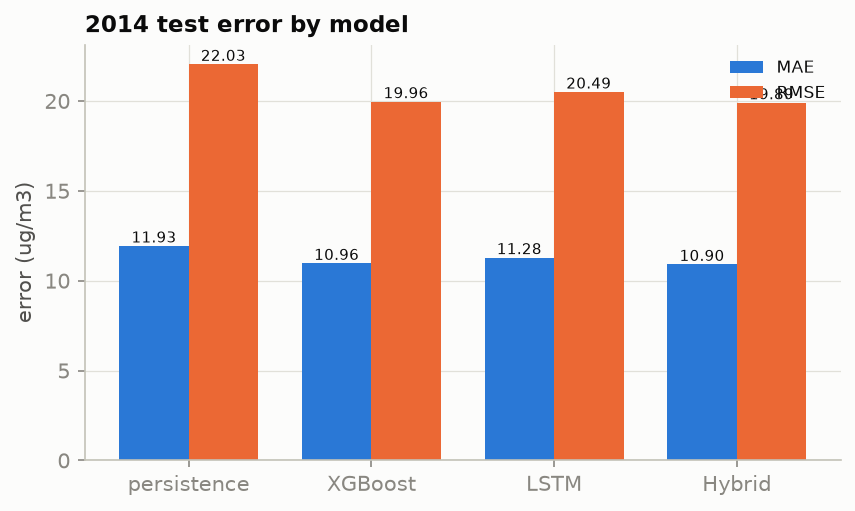
\includegraphics[width=\linewidth]{dl_06_hybrid_compare.png}
\end{columns}
\end{frame}

\begin{frame}{Is it significant? (Diebold--Mariano, 2014)}
\begin{columns}
\column{0.52\textwidth}
\begin{tabular}{llc}
\toprule
Comparison & Loss & $p$ \\
\midrule
LSTM vs persistence & sq.\ & $3\times10^{-8}$ \\
LSTM vs XGBoost & abs.\ & $2\times10^{-5}$ \\
Hybrid vs XGBoost & sq.\ & 0.55 \\
Hybrid vs XGBoost & abs.\ & 0.07 \\
\bottomrule
\end{tabular}
\column{0.48\textwidth}
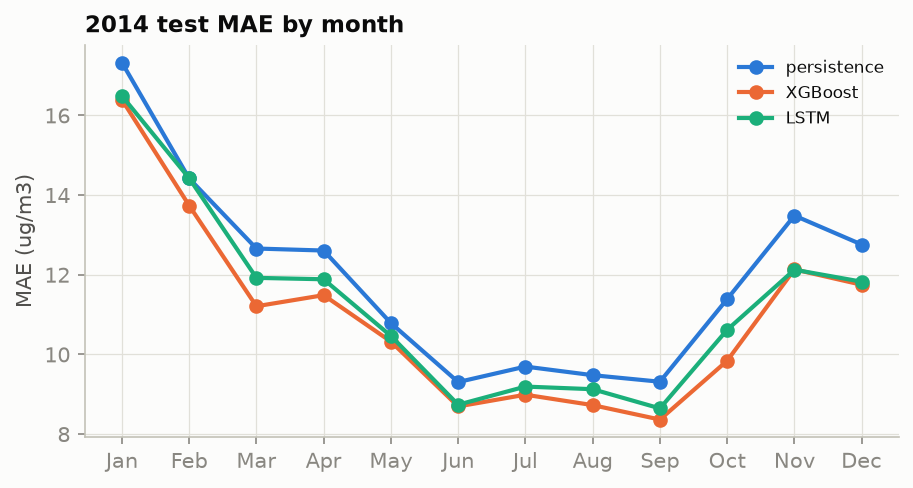
\includegraphics[width=\linewidth]{dl_03_test_monthly.png}
\end{columns}
\begin{itemize}
\item LSTM's gain over persistence is \textbf{real}; XGBoost's edge over the LSTM is \textbf{real}.
\item Hybrid's edge over XGBoost is \textbf{small and not significant} --- we do not overstate it.
\end{itemize}
\end{frame}

\begin{frame}{Where the hybrid helps --- and the wall}
\begin{columns}
\column{0.5\textwidth}
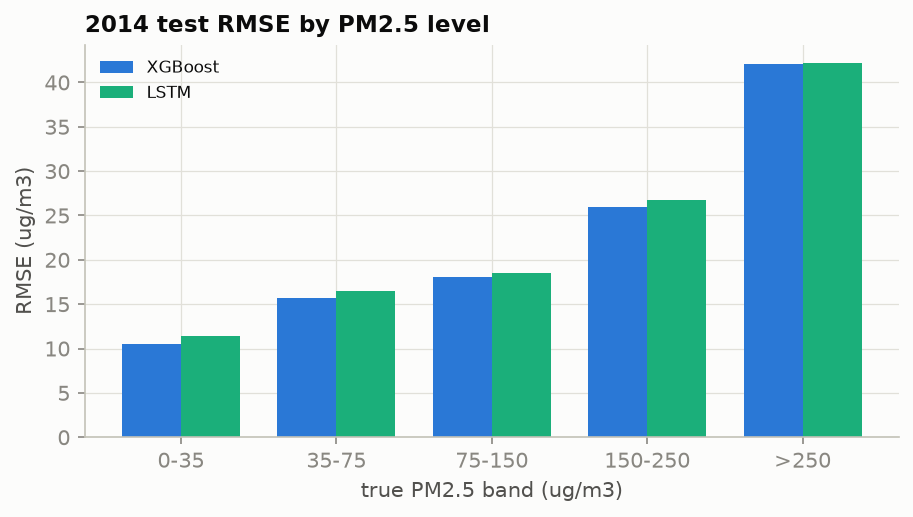
\includegraphics[width=\linewidth]{dl_04_test_by_level.png}
\column{0.5\textwidth}
\begin{itemize}
\item Hybrid improves XGBoost in the \textbf{three higher bands} (75--150, 150--250, $>$250 \ugm{}).
\item Extreme band $>250$: MAE 23.53 vs 23.92 --- the LSTM's different errors pull spikes down.
\item But \textbf{no model solves the extreme}: RMSE $\approx$ 42 \ugm{} for all three (41.6 / 42.0 / 42.2).
\item Same wall Phase~1 hit: rare, sudden spikes remain hardest.
\end{itemize}
\end{columns}
\end{frame}

\begin{frame}{Conclusions --- an honest result}
\begin{itemize}
\item The LSTM learns useful temporal structure from \emph{raw} history and significantly beats the baselines (test MAE 11.28 vs 11.93 \ugm{}).
\item It does \textbf{not} overtake the feature-engineered XGBoost at 1~h --- the problem is dominated by short-range persistence.
\item The hybrid is the best single model (MAE 10.90, $R^2$ 0.955), helping most at high pollution; its edge is modest and not significant --- but it was frozen on validation and still generalised.
\item \textbf{Good DL practice:} windowed inputs with no leakage, training-only scaling, proper regularisation, a fair comparison, and honesty about where deep learning did \emph{not} win.
\item \textbf{Future:} TCN alternative; tail-weighted loss; operational weather forecasts; AQI-category output.
\end{itemize}
\end{frame}

\end{document}
